% #############################################################################
%															Hinderniskarte und Lokalisierung
% #############################################################################
\chapter{Hinderniskarte und Lokalisierung}
\label{lokalisierung_cha}
% ********************************************************************************
% 										Aufgabenstellung
% ********************************************************************************
\section{Aufgabenstellung}
\label{lokalisierung_aufgabenstellung_sec}
\authorsection{\editorandreas}
% -----------------------------------------------------------------------------
%													Lokalisierung
\subsection{Lokalisierung}
Die Aufgabe der Lokalisierung, im Kontext der Robotik, ist die Bestimmung der
Roboter Pose, welche die Position und Orientierung des Roboters in seiner Umgebung vollständig beschreibt.
 Um Bahnplanung und Steuerung zu ermöglichen muss die Pose des Roboters bekannt sein,
 damit sich dieser gefahrlos fortbewegen und sicher mit der Umwelt interagieren kann.
 Für einen Menschen ist die Lokalisierung selbstverständlich, für einen Roboter
 stellt sie allerdings eine Herausforderung dar.
 Aufgrund einer unbekannter Startposition oder von Messungenauigkeiten während
 der Fortbewegung, kann die Pose eines Roboters nur in den seltensten Fällen
 genau bestimmt werden.
 Von lokaler Lokalisierung wird gesprochen wenn die aktuelle Pose des Roboters
 in seiner Umwelt bekannt ist und bei einer Positionsänderung des Roboters diese
 fortlaufend aktualisiert wird, um sie auf dem neusten Stand zu halten. Hier
 werden Schätzungen der Bewegung aufgrund der Odometrie Sensorik mit Hilfe von weiteren Daten zur Posenbestimmung korrigiert. Dieses Vorgehen soll eine Aufsummierung von Fehlern bei der
 Schätzung der Bewegung durch die Odometrie verhindern. Im Gegensatz dazu ist
 bei der globalen Lokalisierung die aktuelle Pose des Roboters in seiner Umwelt
 nicht bekannt und muss zum Beispiel anhand von Kartenmaterial geschätzt werden.
 Man sieht leicht ein, dass bei dieser Art der Lokalisierung die Initiale
 Schätzung einen beliebig großen Fehler aufweisen kann.
 Nach dieser Einführung sollte klar geworden sein das es notwendig
 ist eine Lokalisierung durchzuführen um es unserem Roboter zu
 ermöglichen sich fortzubewegen.
% -----------------------------------------------------------------------------
%													Hinderniskarte
\subsection{Hinderniskarte}
Abgesehen von der Lokalisierung gibt es noch einen weiteren Grund warum es für einen mobilen Roboter unumgänglich ist,
 dass eine interne Repräsentation seiner Umgebung existiert. Karten, die zur Lokalisierung eingesetzt werden,
 enthalten meist nicht alle statischen Hindernisse, da diese Karten zu einem gewissen Zeitpunkt erstellt wurden und
 in der Zwischenzeit wahrscheinlich neue Objekte hinzugekommen oder bereits Vorhandene versetzt worden sind.
 Außerdem enthalten solche Karten offensichtlich keine Hindernisse die sich bewegen können, wie beispielsweise Menschen.
 Ein Hindernis ist ganz allgemein ein Bereich der von dem Roboter nicht befahren werden kann. Eine Darstellung der Hindernisse
 relativ zur Roboterpose wird als Hinderniskarte bezeichnet. Eine solche Karte
 kann zum Beispiel mit Hilfe von Laser- oder Kameradaten erstellt werden.
 Eine Kombination des Materials mehrerer Sensoren ist normalerweise das Sinnvollste,
 da Laser beispielsweise keine negativen Hindernisse erkennen können.
 Als negative Hindernisse werden Bereiche bezeichnet die im Vergleich zur
 gegenwärtigen Position eine geringere Höhe aufweisen.
 Ein Beispiel für ein solches Hindernis ist eine Treppe in ein tiefer gelegenes
 Stockwerk. Das Erstellen einer Hinderniskarte ist aus den oben genannten
 Gründen essentiell um eine Bahnplanung für einen mobilen Roboter
 durchführen zu können.
% -----------------------------------------------------------------------------
%													Virtual protective Field
\subsection{Virtual protective Field}
Die Aufgabe der Bahnplanung besteht darin auf Grundlage der Lokalisierung und der Hinderniskarte einen Weg zu einer
 bestimmten Position zu finden. Danach wird dieser Weg vom Roboter abgefahren. Allerdings kann es während dem Abfahren der gefundenen
 Route Aufgrund eines Hindernisses, dass sich in den Weg des Roboters bewegt bevor erneut geplant werden kann oder
 schlicht Aufgrund eines Fehlers in der Planung dazu kommen, dass der Roboter mit einem Hindernis kollidiert.
 Daher wird eine Möglichkeit benötigt auf einer tieferen Ebene wie der Bahnplanung das unbeabsichtigte kollidieren mit einem Hindernis
 zu verhindern. An dieser Stelle kommt das sogenannte „Virtual protective Field“ ins Spiel, von welchem ein Bereich um den Roboter auf
 Hindernisse überprüft und beim Auffinden eines Solchen ein Signal erzeugt wird, damit der Roboter gestoppt werden kann bevor er
 auf das Hindernis trifft. Dieser Bereich muss mit der Geschwindigkeit des
 Roboters wachsen bzw. schrumpfen so das sichergestellt ist, dass auf jeden
 Fall eine Kollision verhindert werden kann.
% ********************************************************************************
% 										Grundlagen Lokalisierung
% ********************************************************************************
\section{Grundlagen Lokalisierung}
\label{lokalisierung_grundlagen_sec}
\authorsection{\editoranne}
\begin{flushright}\textit{Einige Abschnitte in Anlehnung an das oder aus dem Projektwiki von Dirk~Toewe}\end{flushright}
% -----------------------------------------------------------------------------
%													Lokalisierung
\subsection{Lokalisierung}
Um die im vorangegangenen Abschnitt vorgestellten Aufgaben und Ziele umzusetzen, gibt es verschiedene Möglichkeiten. Wir gehen nun etwas detailierter auf grundlegende Verfahren ein, die für die Durchführung einer Positionsbestimmung von Nutzen sind.
 
\subsubsection{Odometrie}
Die erste vorgestellte Methode zur Positionsbestimmung ist die Odometrie. Dieser aus dem griechischen kommende Begriff steht sinngemäß für ''Wegmessung'' und beschreibt im Wesentlichen schon die Hauptaufgabe. Die Odometrie umfasst die technischen Einrichtungen, die während des Betriebes des Roboters die zurückgelegte Wegstrecke ausmessen.

Ein sehr einfacher und dennoch effektiver Ansatz zur Wegbestimmung ist die Verwendung von Schrittzählern. Bewegt sich der Roboter mittels Beinen fort, wird die Anzahl der gemachten Schritte gezählt. Werden dagegen Rädern  zur Fortbewegung genutzt, können schwarz-weisse Musterscheiben angebracht werden. Diese werden mittels einem oder mehrerer Sensoren abgetastet. Eine einfache, zumeist lineare, Abbildung ermittelt aus der Anzahl der schwarzen und weissen Flächen die zurückgelegte Wegstrecke. Es kann anschließend relativ zur Ausgangpose eine neue Roboterpose angegeben werden.

\begin{figure}[h]
\center
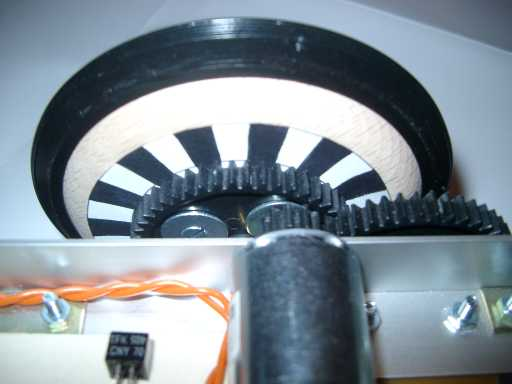
\includegraphics[scale=0.5]{graphics/odo_einbau.jpg}
\caption{\label{fig:Odo_Einbau} Beispiel einer eingebauten Musterscheibe an einer Radachse\citep{odom}}
\end{figure}

Die Vorteile liegen bei diesem Ansatz in der Einfachheit der Konstruktion. Der benötigte Aufwand zur Installation, bzw. Implementation ist nicht sehr hoch und auch nach dem Einbau ist der Rechenaufwand vernachlässigbar gering, da keine komplizierten Funktionsberechnungen nötig sind. Die Nachteile der Methode beruhen vor allem auf den Fehlern, die mit dieser Methode entstehen. Ist der Boden uneben oder besitzt zu viel Schlupf sind die Radumdrehungen nicht mehr konsistent zur zurückgelegten Strecke. Auch die Annahmen über die Rad- und Fahrgestellgeometrie können Ungenauigkeiten enthalten. So ist zum Beispiel ein Rad nicht gänzlich rund oder die Radabstände wurden ungenau gemessen oder haben sich durch Verschleiß und Benutzung verändert. Zu diesen Nachteilen, die an sich schon eine fehlerhafte Wegbestimmung nach sich ziehen, kommt noch erschwerend hinzu, dass die Odometrie keine rückgekoppelte Methode ist, sich eingeschlichene Fehler selbstverständlich mit dem Betrag der zurückgelegten Wegstrecke aufsummieren und dies auch noch abhängig von der aktuellen Situation in unterschiedlichem Maße. Der Fehler kann also nicht fest mit ein- oder gar gänzlich herausgerechnet werden. Des Weiteren kann nur eine relativ zu einer Ausgangspose berechnete neue Roboterpose angegeben werden. Diese Methode eignet sich daher nur für eine lokale, nicht jedoch für eine globale Lokalisierung. Die Ursprungsposition muss dem Roboter von aussen mitgeteilt werden.

\subsubsection{Kartenbasierte Lokalisierung}

Ist eine Karte der Umgebung gegeben, in der sich der Roboter aufhält, so kann mittels geeigneter Sensordaten die Roboterpose geschätzt, bzw. eindeutig bestimmt werden. Eine Möglichkeit besteht darin, Laser an dem Roboter anzubringen und mittels Abstandsdaten Gegenstände, Wände und Flächen zu erkennen. Dazu wird aus einer Punktwolke eine Menge von geometrischen Figuren, wie zum Beispiel Kanten extrahiert. Diese werden mit den Kartenmaterial abgeglichen und man erhält im schlechten Fall mehrere mögliche Positionen, im optimalen Fall eine eindeutige Position an der sich der Roboter aktuell befindet.

Hierbei wird immer die aktuelle Roboterpose berechnet ohne auf vorhergehende Roboterposen angewiesen zu sein. Dies ist vorteilhaft, da sich im Laufe des Betriebes keine Fehler akkumulieren können und man nicht einmal eine Ausgangspose benötigt. Allerdings ist der Roboter auf möglichst detailgetreues Kartenmaterial angewiesen, welches selbstverständlich aktuell gehalten werden muss. In einer Umgebung in der keine markanten Stellen zu finden sind, wird die Zahl der möglichen Roboterposen eventuell unangenehm hoch sein. Dazu kommen die Nachteile der Technik, die verwendet wird um Informationen über die Umwelt zu erhalten. Bei einem Laser muss darauf geachtet werden, dass er freie Sicht hat und gerade am Roboter angebracht ist. Zusätzlich kann der Laser fehlerhafte Daten zurückliefern, wenn er auf spiegelnde, glatte Flächen trifft, durch eine Glaswand hindurchsieht oder von sich bewegenden Gegenständen umgeben ist.  

\subsubsection{Landmarkbasierte Lokalisierung}

In einer bekannten Umgebung können Landmarks (\gls{qr}-Codes, Bodenlinien,
 \gls{gps}-Satelliten) angebracht werden. Diese können durch Sensoren
 am Roboter wiedererkannt werden und ermöglichen die Lokalisierung
 z.B. mittels Triangulierung.

\begin{itemize}
  \item Vorteile:
  \begin{itemize}
    \item (durchschnittlicher) Fehler niedrig
    \item Zuverlässig (max. Fehler niedrig)
    \item Keine Fehlerakkumulation über Zeitverlauf
  \end{itemize}
  \item Nachteile:
  \begin{itemize}
    \item Landmarks notwendig
    \item Landmarks müssen von überall sichtbar sein
    \item Kartenmaterial u.U. notwendig
   \end{itemize}
\end{itemize}

Um die Nachteile der verschiedenen Lokalisierungsmethoden zu
 verringern werden in der Regel mindestens zwei Methoden miteinander
 kombiniert. Aufgrund der einfachen Implementierung und der geringen
 Störanfälligkeit ist meistens die Odometrie in Kombination mit
 anderen Systemen vorzufinden. Bei Verwendung mehrerer Methoden sind
 dementsprechend viele fehlerbehaftete Annahmen der aktuellen
 Roboterpose gegeben. Im Folgenden wollen wir zwei unterschiedliche
 Verfahren vorstellen, welche aus diesen Annahmen bestmöglich die
 aktuelle Roboterpose bestimmen.
 
\subsubsection{Kalman-Filter}

Das Kalman-Filter ist eine der wichtigsten Entdeckungen des letzten Jahrhunderts, entwickelt von dem Ingenieur Rudolf E. Kalman.
Sind nun eine Reihe von Messwerten in Form von möglichen Roboterposen gegeben, die von unterschiedlichen Messverfahren herrühren und mit einem Rauschen behaftet sind, so schätzt das Kalman-Filter eine aktuelle Roboterpose.
Die Grundidee sieht man an der Ausgangsgleichung \[ \hat{x}_k = G_k v_k + (1-G_k) \hat{x}_{k-1}, \] wobei \(\hat{x}_k\) der aktuelle und  \(\hat{x}_{k-1}\) der vorherige Schätzwert sei. \(G_k\) das sogenannte Kalman-Gain und \(v_k\) der aktuelle Messwert, der allerdings verrauscht ist und daher mit einem Fehler behaftet. Das Kalman-Gain gewichtet die bisherigen Messwerte in Bezug auf den akuell gemessenen Wert und berechnet daraus den aktuellen Schätzwert \(\hat{x}_k\).
Das Ziel ist einen möglichst guten Schätzwert \(\hat{x}_k\) zu finden, der den Wert \(v_k\) am besten beschreibt.
In den Iterationsschritten wechseln sich nun Prädiktion und Korrektion ab: Aus den letzten \(k-1\) Messungen wird ein vorraussichtlicher Wert \(k\) vorhergesagt (''Prädiktion''). Nachdem die \(k\)te Messung stattgefunden hat, man also eine Information mehr dazu gewonnen hat, wird der Messwert zum Zeitpunkt \(k\) verbesserert (''Korrektur''). Dabei kann in jedem Schritt aus den gemachten Beobachtungen das Kalman-Gain neu angepasst werden.

\subsubsection{Partikel-Filter}

Als Alternative zum Kalman-Filter existiert die Sequentielle Monte-Carlo-Methode. Auch bekannt als Partikel-Filter. Mit Hilfe dieser Methode können ebenfalls kontinuierlich Ort und Geschwindigkeit, insbesondere eines autonomen Roboters, ermittelt werden, obwohl nur ungenaue Messwerte vorliegen.
Ist das Prozessmodell nicht linear oder sind die äußeren Einflüsse, die zu fehlerhaften Messwerten führen nicht normalverteilt, kann auch nicht von einer Normalverteilung des zu schätzendes Zustandes ausgegangen werden. Eine Normalverteilung hat die Eigenschaft nur ein Maxima aufzuweisen und somit nur einen möglichen besten Zustand zurück zu liefern. Liegt diese nicht vor, muss angenommen werden, dass die Wahrscheinlichkeitsdichte mehrere Maxima aufweist, das heisst, das mehrere mögliche Zustände in Frage kommen, als die Besten und Wahrscheinlichsten zum gegenwärtigen Zeitpunkt zu gelten.
Diese unbekannte, aber gerade aktuelle Warscheinlichkeitsdichte auf dem Zustandsraum soll nun geschätzt werden, um daraus den wahrscheinlichsten Zustand zu schätzen. Dazu wird eine Menge von Partikeln erzeugt. Jeder Partikel ist dabei ein Paar aus Gewicht und einem Punkt im Zustandsraum. Die Menge der Partikel repräsentiert die Wahrscheinlichkeitsdichte.
Jedem Partikel wird dann eine mögliche Lösungskurve zugeordnet und je besser diese zu den tatsächlichen Messwerten passt, desto mehr wird das Gewicht des Partikels angepasst. Im Laufe der Messungen verbessert sich somit die Schätzung der Wahrscheinlichkeitsdichte, welches durch Methoden der nichtparametrischen Dichteschätzung erfolgt.\citep{rob3}

 
% ********************************************************************************
% 										Umsetzung
% ********************************************************************************
\section{Umsetzung}
\label{lokalisierung_umsetzung_sec}
\authorsection{\editorandreas}
\begin{flushright}\textit{Einige Abschnitte aus dem Projektwiki übernommen deren
Autor: Dirk~Toewe}\end{flushright}
% -----------------------------------------------------------------------------
%													Lokalisierung
\subsection{Lokalisierung} 
In diesem Abschnitt wollen wir uns mit der eigentlichen Umsetzung der
 Lokalisierung beschäftigen. Wie sie wahrscheinlich schon aus Kapitel
 \ref{grundlagen_cha} wissen, verfügen die beiden Roboter \gls{hollie} und
 \lstinline{Odete} über sehr ähnliche Sensoren, die zur Lokalisierung verwendet
 werden können. Der Roboter \lstinline{Odete} weist 2 Winkelencoder und einen 270 Grad Sick
 Laserscanner (Scheibenförmiger Scan) auf.
 \gls{hollie} verfügt über 2 Winkelencoder und zwei
 270 Grad Sick Laserscanner.
 Offensichtlich musste, um ein sicheres Fortbewegen des Roboters zu
 gewährleisten, für das \lstinline{Odete}-Projekt ebenfalls eine Lokalisierung implementiert werden.
 Im Folgenden wollen wir kurz auf die grundlegende Idee für den Aufbau der
 Gruppen und Module bezüglich der Lokalisierung eingehen.
 Die verwendete \lstinline{MCA2}-Struktur der \lstinline{Odete} basiert auf
 einem bestimmten Paradigma.
 Ziel ist es eine hohe Flexibilität zu erreichen. Sensoren und Plattformen sollen
 beliebig kombinierbar sein. Wir entschieden uns daher dazu diese Struktur auch
 beim \lstinline{SegwayOmni}-Projekt weiterzuführen. Dadurch konnten alte
 Programmstrukturen übernommen und/oder adaptiert und außerdem dieselbe
 Flexibilität wie im \lstinline{Odete}-Projekt erreicht werden. Daher gelten die folgenden Erläuterungen
 zur Lokalisierung auch fast uneingeschränkt für beide Robotersysteme.
 Zur Positionsschätzung wird bei beiden Systemen eine Kombination aus
 kartenbasierter Lokalisierung und Odometrie verwendet. Die Schätzwerte aus beiden Messungen werden mit einem Kalman-Filter zu einer
 Synthese geschätzt. Dem Kalman-Filter ist eine Queue (\gls{fifo}) vorgeschaltet, in der jede Schätzung
 mit einem Timestamp registriert wird. So können die Messwerte in zeitlich korrekter Reihenfolge
 eingerechnet werden, selbst dann, wenn sie nach der Verarbeitung in einer anderen Reihenfolge
 im Kalman-Filter registriert werden. Die für die Odometrie benötigte Winkelschrittmessung der Räder wird direkt
 von der Segway-Antriebsplattform geliefert.
 Es wird angenommen, dass der Fehler linear ansteigt mit der durch den Reifen zurückgelegten Strecke.
 Falls eine gute Schätzung aus der kartenbasierten Lokalisierung in den Kalman-Filter übergeben wird,
 wird die Pose korrigiert und der Odometriefehler wieder gesenkt.
 Nach den Erläuterungen dazu wie die Lokalisierung durchgeführt wird wollen wir
 jetzt die beteiligten Gruppen und Module etwas näher betrachten. 

\begin{description}
\item[HAL(Hardware abstraction Layer)] Die \lstinline{Hal}-Gruppe ist für
 plattformabhängige Hardware zu\-ständig.
 Mit der Plattform sind jene Hardwarekomponenten gemeint, die in der Regel nicht getauscht werden 
 (Rechner, Omnidirektionaler Antrieb, Akummulatoren).
 In \lstinline{MCA2} umfasst die \lstinline{Hal} die Bewegungsplattformen, die dazugehörigen
 Winkelencoder und die Posenerfassung (nicht Posenberechnung) des Roboters. Die \lstinline{Hal} ist eine Abstraction Layer in dem Sinne, dass zwischen einer Simulierten
 Hardware und der tatsächlichen Hardware gewechselt werden kann, ohne das andere
 \lstinline{MCA2}-Gruppen angepasst werden müssen.
 Prinzipiell können sogar die Plattformen (Omnidirektional <-> Differentiell) ausgetauscht werden. Die Odometrie hängt
 direkt mit der Antriebsart zusammen und findet deswegen in der \lstinline{Hal} statt.
 Auch die Kalman-Filterung findet in dieser Gruppe im
 \lstinline{AbsoluteCoordinatesMecanumKLF}-Modul statt (KLF = KalmanFilter). Für
 eine Darstellung der Gruppe siehe Abbildung \ref{fig:segwayHal}.
\item[SAL(Scanner abstraction Layer)] Die \lstinline{Sal}-Gruppe umfasst alle ``angebauten''
Scanner, nicht aber in Plattform integrierte Scanner (Winkelencoder).
 Im Sinne der Abstraction Layer können auch hier Hardware- und
 Simulationsversion der \lstinline{Sal} ausgewechselt werden, siehe Abbildung
 \ref{fig:SegwayOmniSal}
\end{description}
\begin{figure}[h]
\center
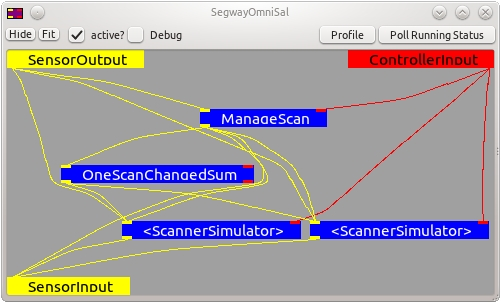
\includegraphics[scale=0.7]{graphics/SegwayOmniSal.jpg}
\caption{\label{fig:SegwayOmniSal} SegwayOmniSal}
\end{figure}

Diese Beiden Gruppen realisieren also unter anderem die erste benötigte
 Abstraktion der Sensordaten sowie eine Simulation für den Testfall. Zu beginn
 des Projektes existierte bereits eine \lstinline{Hal} Gruppe im
 \lstinline{SegwayOmni}-Projekt, allerdings war darin noch keine kartenbasierte
 Positionskorrektur durch den Kalman-Filter realisiert. Diese Funktionalität und
 die \lstinline{Sal}-Gruppe wurden einige Zeit später durch einen unserer Betreuer,
 Jan Oberländer implementiert. Da wir Anfangs nicht wussten
 welche Funktionalitäten von uns implementiert werden mussten hatte unserer Gruppe einige Schwierigkeiten
 einen Einstieg zu finden. Dies äußerte sich vor allem darin, dass wir zu Beginn des Praktikums viel Zeit damit
 verbrachten zu versuchen uns in alle Gruppen und Module einzuarbeiten.

Nach der Feststellung der benötigten Anpassungen an die vorhandenen Gruppen und
 Module des \lstinline{Odete}-Projekts wurden diese adaptiert. Außerdem wurden
 Erweiterungen integriert damit eine beliebige Menge von Scannern genutzt werden
 kann.
 Eine Parametrisierung über einen Multiplexer und ein XML-Config-File
 ermöglichen eine Anpassung auf eine neue Sensor-Anordnung. Abschließend erfolgt
 nun noch eine detailliertere Erläuterung der für die kartenbasierte
 Lokalisierung nötigen Schritte und der involvierten Gruppen und Module. Die kartenbasierte Lokaliserung
 findet in den \lstinline{MCA2}-Gruppen \lstinline{LlSP} und \lstinline{HLSP}
 statt. Die Laserscanner-Daten dazu werden wie schon erörtert aus der
 \lstinline{SAL}-Gruppe bezogen.
 Für eine Darstellung der beiden Gruppen im \lstinline{Mcabrowser} siehe
 Abbildung \ref{fig:Llsp} und \ref{fig:Hlsp}.
 
\begin{figure}[h]
\center
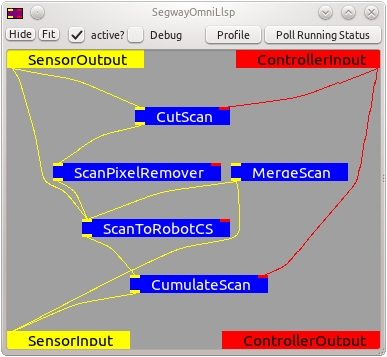
\includegraphics[scale=0.7]{graphics/Llsp.jpg}
\caption{\label{fig:Llsp}Llsp -- Low Level Scanner Processing}
\end{figure}

\begin{figure}[h]
\center
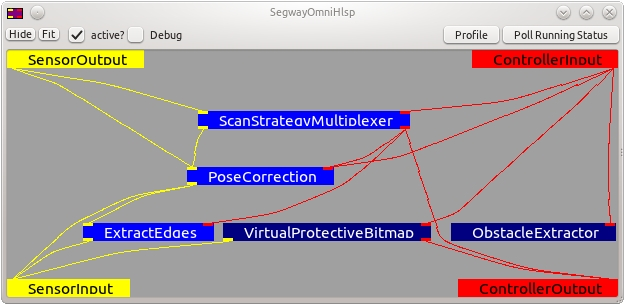
\includegraphics[scale=0.7]{graphics/Hlsp.jpg}
\caption{\label{fig:Hlsp}Hlsp -- High Level Scanner Processing}
\end{figure}
 
\begin{description}
\item[LLSP(Low Level Scanner Processing)] Die \lstinline{LLSP} dient der
Verarbeitung der Scanner Rohdaten. Im Gegensatz zur \lstinline{HLSP} macht die
\lstinline{LLSP} keine logische Auswertung der Scannerdaten.
 Es werden lediglich grundlegende Operationen auf die einzelnen Messwerte angewandt
 (Koordinatentransformationen, Löschen ungültiger Werte, ...).
\item[HLSP(High Level Scanner Processing)] In der \lstinline{HLSP} werden
logische Operationen auf die\\ Messwerte angewandt (Kantenextraktion,
Posenkorrektur-Schätzung).
\begin{itemize}
  \item Der \lstinline{ScanStrategyMultiplexer} dient als zentrale Schaltstelle
  für die Controllerinputs der \lstinline{HLSP}-Module.
  Über einen einzelnen Controllerinput des \lstinline{ScanTrategyMultiplexer}
  kann ein Setup geladen werden, welches die Controllerinputs der einzelnen
 \lstinline{HLSP}-Module setzt.
\end{itemize}
\end{description}

Die kartenbasierte Posen-Schätzung wird in den folgenden Schritten ermittelt:

\begin{enumerate}
  \item Scheibenförmiger Laser-Scan der Umgebung parallel zur Fahrbahn\\
    	Gruppe: \lstinline{SAL}\\
    	Ergebnis: Winkel-Abstand-Paare (Polarkoordinaten)\\
  \item Koordinaten-Transformation: polare Sensorkoordinaten -> kartesische
  		Sensorkoordinaten\\
  		Gruppe: \lstinline{LlSP}\\
    	Modul: \lstinline{ScanToRobotCS}\\
    	Ergebnis: XY-Punkte (kartesische Sensorkoordinaten)\\
  \item Koordinaten-Transformation: kartesische Sensorkoordinaten -> kartesische
  		Roboterkoordinaten\\ 
  		Gruppe: \lstinline{LlSP}\\
  		Modul: \lstinline{MergeScan}\\
  		Ergebnis: XY-Punkte (kartesische Roboterkoordinaten)\\
  \item Löschen von Punkten mit zu hohem Abstand oder schlechter Auflösung\\
    	Gruppe: \lstinline{LlSP}\\
    	Modul: \lstinline{CutScan}\\
    	Ergebnis: XY-Punkte mit gültigem Abstand\\
  \item Extraktion/Schätzung von Kanten aus der Punktemenge\\
    	Gruppe: \lstinline{HlSP}\\
    	Modul: \lstinline{ExtractEdges}\\
    	Ergebnis: Liniensegmente\\
  \item Vergleich der Kanten mit der Karte und Schätzung einer Pose samt
  		Fehlerkovarianz\\ 
  		Gruppe: \lstinline{HlSP}\\
    	Modul: \lstinline{PoseCorrection}\\
    	Ergebnis: X,Y,Gierwinkel-Schätzung + Fehlerkovarianz\\
\end{enumerate}

% -----------------------------------------------------------------------------
%													Hinderniskarte
\subsection{Hinderniskarte}
\label{hinderniskarte_subsec}
\authorsection{\editorandreas}
 Im Gegensatz zur Lokalisierung gab es für die von uns gewünschte Lösung dieser
 Aufgabenstellung noch keine Gruppen oder Module von älteren Projekten. Aus
 diesem Grund war es notwendig im Vorfeld intensivere Überlegungen über die möglichen
 Umsetzungen und Repräsentationen anzustellen.
 Nach einigen Diskussionen entschieden wir uns für die Nutzung von
 Bildverarbeitungs"=Modulen aus der \lstinline{SenseIVT}-Bibliothek
 und einer Repräsentation der Hinderniskarte durch ein
 Schwarzweiß-Bitmap. Der Grund für diese Wahl lag vor
 allem an der guten Visualisierung, die dadurch erhalten werden kann, außerdem wird eine einfache
 Anpassung und die Verwendung von Standard-Filtern ermöglicht.
\begin{figure}[h]
\center
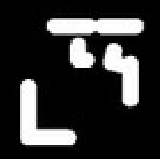
\includegraphics[scale=0.7]{graphics/hinderniskarte.jpg}
\caption{\label{fig:hinderniskarte} Hindernisskarte als Schwarzweiß-Bitmap}
\end{figure}
 In Abbildung \ref{fig:hinderniskarte} ist ein Beispiel eines solches Bitmaps
 zu sehen. Mit der Semantik, dass weiße Areale Hindernisse darstellen und schwarze Bereiche entweder befahrbar
 oder von dieser Position aus nicht einsehbar sind. Diese von uns gewählte Abbildung der Werte
 auf die entsprechenden Bedeutungen ist allerdings beliebig und hat keinen besonderen Grund.
 Die Roboterposition ist der Mittelpunkt der Karte. Bevor Hindernisse in eine solche Karte eingezeichnet werden
 können müssen sie offensichtlich zuvor durch Sensoren detektiert worden sein. Es lag nahe die Laserdaten,
 welche auch zur Lokalisierung eingesetzt und bereits in geeigneter Form vorhanden waren zu nutzen.
 Da ein Roboter in der Realität eine größere Fläche als ein Punkt aufweist entschieden wir uns bereits an dieser
 Stelle zu einer Expansion der Hindernisse auf Robotergröße, damit solche Berechnungen an anderer Stelle vermieden
 werden können.
\begin{figure}[h]
\center
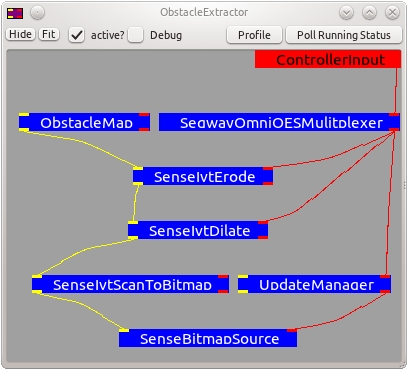
\includegraphics[scale=0.8]{graphics/ObstacleExtractor.jpg}
\caption{\label{fig:obstacleExtractor} Gruppe \lstinline{ObstacleExtractor}}
\end{figure}
 In Abbildung \ref{fig:obstacleExtractor} ist die die Gruppe
 (\lstinline{ObstacleExtractor}), durch welche die gewünschte Funktionalität implementiert wurde zu sehen.
 Im Folgenden wollen wir auch hier die einzelnen Module kurz vorstellen:

\begin{description}
\item[SegwayOmniOESMultiplexer] Dieses Module ermöglicht es die anderen Module der Gruppe zu steuern.
 Hier kann durch einen Controllerinput die gesamte Gruppe aktiviert oder deaktiviert werden.
 Außerdem kann die Größe der Erode- und Dilate-Filtermasken manipuliert werden.
\item[UpdateManager] Dieses Module ist ein Teil der
\lstinline{SenseIvt}-Bibliothek und dient dazu die Aktualisierung der Quelldaten
zu beeinflussen.
\item[SenseBitmapSource] Auch dieses Modul ist ein abgewandelter Teil der
\lstinline{SenseIvt}-Bibliothek, es dient in unserem Fall dazu ein, in einem
 XML-Config-File spezifiziertes schwarzes Bitmap zu laden.
 Dafür stehen unterschiedliche Größen zur Verfügung.
\item[SenseIvtScanToBitmap] Hier werden die Hindernisse aus den Laserdaten extrahiert und auf Robotergröße expandiert.
\item[SenseIvtDilate] Ein Dilate-Filter.
\item[SenseIvtErode] Ein Erode-Filter. Zusammen mit dem vorigen Dilate-Filter
wird hier eine Schlie\-ßen-Operation ausgeführt.
\item[ObstacleMap] Diese Modul dient dazu mit Hilfe eines Plugins des
\lstinline{Mcabrowser} die resultierende Hinderniskarte betrachten zu können.
\end{description}

% -----------------------------------------------------------------------------
%													Virtual protective Field
\subsection{Virtual protective Field}
\label{sec:vpf}
Ein Virtual protective Field, was die letzte von uns zu lösenden Aufgabe
darstellte war bereits im \lstinline{Odete}-Projekt realisiert,
 allerdings war dieses lediglich für einen Differentialantrieb implementiert.
 Nach einer Begutachtung des bestehenden Moduls entschieden wir uns dafür
 dieses nicht für omnidirektionale Bewegung anzupassen sondern eine neue Gruppe mit der gewünschten Funktionalität
 zu erstellen, da uns dies effizienter erschien. Die Wahl der für die Umsetzung benötigten Primitiven viel, aufgrund
 der von uns gewonnen Erfahrungen mit den Bildverarbeitungs-Modulen und der Möglichkeit die bereits bestehende
 Hinderniskarte auszunutzen auch hier auf die \lstinline{SenseIVT}-Bibliothek.
 Als Repräsentation wurde wieder ein Schwarzweiß-Bitmap gewählt. Auf Anfrage der
 Bahnplanungs und Steuerungs Gruppe implementierten wir 3 unterschiedliche
 Virtual protective Fields siehe Abbildung \ref{fig:virtualprotectivefields}.
 \begin{figure}[h]
\center
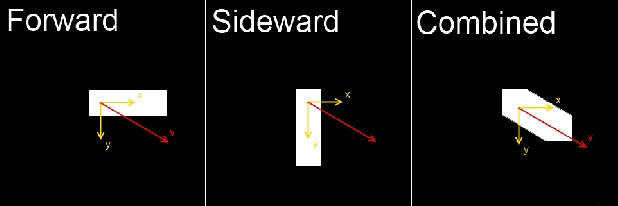
\includegraphics[scale=0.5]{graphics/virtualprotectivefields.jpg}
\caption{\label{fig:virtualprotectivefields} Darstellung der unterschiedlichen Protective
Fields}
\end{figure}
 Die Varianten \emph{Sideward} sowie \emph{Forward} sollen es \gls{hollie}
 ermöglichen eine Bewegung in zumindest eine Richtung durchzuführen wenn die Kombination zu einer Kollision führen würde.
 Die Virtual protective Fields unterliegen einer dynamischen Ausdehnung zum
 Quadrat der Geschwindigkeit um ein erfolgreiches Anhalten vor einer Kollision zu gewährleisten. Aufgrund der Nutzung von Bildverarbeitungs-Modulen
 konnte die Erkennung einer möglichen Kollision durch eine AND-Operation auf der Hinderniskarte und dem entsprechenden
 Virtual protective Field realisiert werden. Sollten nach dieser Operation noch
 weiße Pixel im resultierenden Bitmap vorhanden sein gilt dies als erkannte Kollision. Aufgrund von Fehlern der Laserdaten wird verlangt, dass mehr als ein
 weißer Pixel vorhanden ist, um das Verfahren etwas robuster zu machen.
\begin{figure}[h]
\center
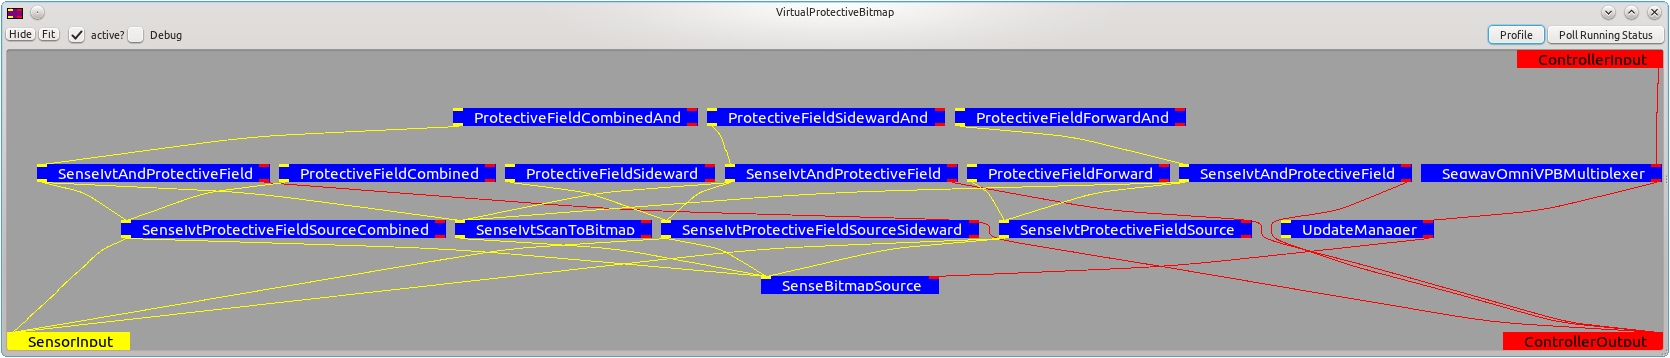
\includegraphics[scale=0.29]{graphics/VirtualProtectiveBitmap.jpg}
\caption{\label{fig:virtualprotectivebitmap} Gruppe \lstinline{VirtualProtectiveBitmap}}
\end{figure}
 Wie bereits in den beiden vorigen Abschnitten  ist auch hier in Abbildung
 \ref{fig:virtualprotectivebitmap} die beschriebene Gruppe dargestellt und es
 folgt eine nähere Betrachtung der Module.
 Wobei wir allerdings nicht erneut näher auf die Module, die bereits zuvor
 vorgestellt wurden eingehen werden.

\begin{description}
\item[SegwayOmniVPBMultiplexer] Ähnlich wie das Modul
\lstinline{SegwayOmniOESMultiplexer} aus dem vorigen Abschnitt werden die
 übrigen Module der Gruppe hier gesteuert und können beispielsweise aktiviert
 beziehungsweise deaktiviert werden.
\item[SenseIvtProtectiveFieldSource] Dieses Modul dient in der jeweiligen
Variation dazu das entsprechende Virtual protective Field in ein schwarzes
Bitmap einzuzeichnen. Wie bereits besprochen ist die Größe des Feldes abhängig
vom Bremsweg und unterliegt einem gewissen Sicherheitspuffer.
\item[SenseIvtAndProtectiveField]  Diese Modul realisiert die AND-Operation zwischen dem jeweiligen
 Virtual protective Field und der Hinderniskarte. Außerdem wird der entsprechende Controlleroutput gesetzt
 sollten nach der Operation noch mehr als 3 weiße Punkte im resultierenden Bitmap vorhanden sein.
\end{description}

Die Module \lstinline{ProtectiveFieldSideward},
 \lstinline{ProtectiveFieldForward} und
 \lstinline{ProtectiveFieldCom-}\lstinline{bined} dienen wie das Modul
 \lstinline{ObstacleMap} aus der \lstinline{ObstacleExtractor}-Gruppe zur Visualisierung, wobei hier die Virtual
 protective Fields dargestellt werden können. Die Module 
 \lstinline{ProtectiveField-}\lstinline{SidewardAnd},
 \lstinline{ProtectiveFieldForwardAnd} und \lstinline{ProtectiveFieldCombinedAnd} können dazu genutzt werden die
 Bitmaps nach der AND-Operation anzuzeigen.
